\documentclass{article}
\usepackage[utf8]{inputenc}
\usepackage{geometry}
\usepackage{graphicx}
\usepackage[hidelinks]{hyperref}

\begin{document}

% \title{Report on Dealing with Uncertainty}
% \author{Ayushi Chaudahry}
% \date{\today}
\begin{titlepage}
    \centering
    \vspace*{1cm}
    
\includegraphics[width=0.6\textwidth]{Logo.jpg} % Replace with your university logo
    \par\vspace{0.5cm}
    {\Huge\textbf{Dealing with Uncertainty}\par}
    \vspace{1.5cm}
    {\Large\textbf{Ayushi Chaudhary}\par}
    \vspace{0.5cm}
    {Student ID: 40224978\par}
    \vspace{2cm}
    {\Large\textbf{SOEN 6841: Software Project Management}\par}
    \vspace{1cm}
    {\large\textbf{Submitted to Professor Pankaj Kamthan}\par} % Replace with your professor's name
    \vfill
    {\large\textbf{Date: 30/10/2023}\par}
\end{titlepage}

\pagenumbering{gobble}
\newpage
\tableofcontents
\newpage
\pagenumbering{arabic}
\addcontentsline{toc}{section}{Abstract}
\section*{Abstract}
In the realm of software engineering, decision-making under uncertainty is a significant challenge, especially when confronted with limited or conflicting information. A systematic approach is essential for navigating these uncertainties, providing a practical guide for effective decision-making. Such a framework not only improves the decision-making skills of professionals and students in the field but also contributes significantly to the success of software projects. The study reveals that in the face of rapidly evolving information, traditional decision-making strategies may become inadequate, necessitating a shift towards more adaptive methods. This adaptability is essential to maintain decision quality amidst dynamic conditions. The results emphasize the importance of embracing uncertainty as an inherent part of the decision-making process, while keeping a clear focus on objectives to guide informed and confident decisions. The study also highlights a variety of techniques, such as scenario planning, prototyping, experimentation, risk management, and collaboration, as effective tools for navigating the complexities posed by uncertainty and risk. Collectively, these insights underscore the necessity for agility and adaptability in decision-making processes within uncertain and continuously changing environments.
\newline
\newline
\textbf{Keywords:}Uncertainty, Decision-making, Adaptive methods, Informed decisions, Risk management, Collaboration, Adaptability, Agility.
% Your abstract content
\newpage

\section{Introduction}

\subsection{Motivation}

An understanding of the decision-making process is critical not only for the explanation of individual behavior but also for the behavior of complex organizations.\cite{vroom1973leadership}
\\
In the ever-changing landscape of managerial responsibilities, decision-making stands out as a critical aspect that leaders must deal with on a daily basis. Managers face a plethora of options, ranging from routine and straightforward to complex and ambiguous. \\
The motivation for this report stems from the realisation that decision-making, especially in the face of uncertainty, poses significant challenges for managers across industries.
The motivation for researching this issue stems from the potential consequences of poor decision-making. Poorly managed uncertainty can lead to misalignment with organisational goals, decreased team morale, and, ultimately, a project or initiative's failure. 
\newline
The purpose of this report is to delve into the strategies and considerations that can enable managers to make effective decisions in the face of uncertainty, while also acknowledging the inherent challenges and providing valuable insights for navigating these complexities.


% Your motivation content
\subsection{Problem Statement}
A key obstacle in decision-making is the need to define explicit challenges and goals. Decisions are less likely to get the necessary buy-in or support if objectives and problem statements are not clearly articulated. This is especially important when making judgements with little or contradictory information. A lack of defined goals can lead to ineffective conversations focusing on minor technicalities or implementation elements (a tendency known as "bikeshedding") rather than achieving an agreement on the decision's underlying need. To successfully handle the issue at hand, it is critical to collect varied perspectives and information from multiple sources inside the organisation, ensuring a well-rounded knowledge of the situation. This strategy aids in connecting decision-making procedures with the organization's actual requirements and goals, allowing for more effective and informed decisions in the face of uncertainty.


% Your problem statement content
\subsection{Objectives}
Enhanced decision-making under uncertainty is crucial for organizational success, emphasizing the need to identify and categorize uncertainties effectively. Employing strategies such as information gathering, risk acknowledgment, flexible planning, and systematic evaluation is key.\cite{forman2001decision} These skills are not only vital for individual leaders but also impact the broader organization, leading to improved strategic outcomes and resilience. Effective decision-making in uncertain conditions has emerged as a critical component of successful leadership, underlining its significance in driving organizational growth and sustainability.
% Your objectives content

\section{Background Material}
\subsection{Difference in Risk and Uncertainty}
 There are three categories of decision-making scenarios:\\
 (a) \textbf{Certainty}, where each action is known to lead invariably to a specific outcome.\\
 (b) \textbf{Risk}, where each action leads to one of a set of possible specific outcomes, each outcome occurring with a known probability. \\
 (c) \textbf{Uncertainty}, where actions may lead to a set of consequences, but where the probabilities of these outcomes are completely unknown.
 \\
 \begin{figure}[h!]
\centering
  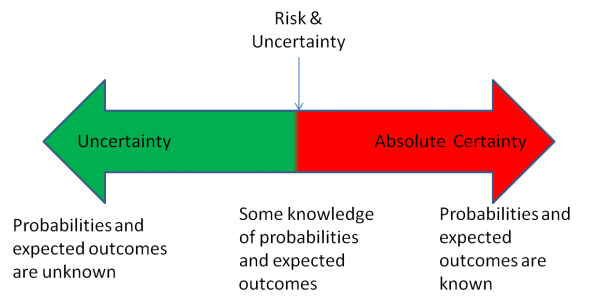
\includegraphics[scale=0.5]{barometer-of-certainty-and-uncertainty-600x300.png}
  \caption{Risk and Uncertainty \cite{Itsomerz2014}}
  % \label{fig:boat1}
\end{figure}
 A risky situation is thus a situation where the outcome is unknown to the decision-maker, i.e. he/she is not sure which outcome will occur and the uncertainty may lead to erroneous choices. 

\subsection{Theoretical Frameworks in Decision Making}
According to \cite{ahmed2012theories}, \textbf{Normative theory} provides a framework for striving towards optimal decision-making, even when faced with incomplete information. \textbf{Descriptive theory}, on the other hand, offers insights into actual decision-making practices and challenges, especially in scenarios where information is ambiguous or incomplete.


\subsection{Types of Uncertainty \& Coping Strategy }
Decision-making often involves navigating through situations where there's an inadequate understanding of the problem, incomplete information available, or when alternatives are not clearly distinguishable. Recognizing and categorizing the type of uncertainty faced is crucial in determining the appropriate response.\cite{LIPSHITZ1997149}
\newline \newline
Effective coping strategies include reducing uncertainty by gathering more information, acknowledging it as part of the process, suppressing it when necessary, preparing for various outcomes (forestalling), and weighing the pros and cons of different options. Decisions often fall into two models: consequential action, based on potential outcomes, and obligatory action, driven by rules or duties (R.A.W.F.S.). Adapting these strategies to specific uncertainties is key, especially for leaders and managers in complex decision-making scenarios.
\subsection{Case Study 1}
\textbf{Embracing Uncertainty in Strategic Decision-Making}\cite{taghavifard2009decision}
\\
\\
\textbf{Company Background}: A multinational, consumer brand company with a focus on outsourcing manufacturing primarily to Asian countries.
\\
\textbf{Challenge}: The company, anticipating a doubling in sales volume, faced key decisions: expand current locations, outsource to a politically unstable country (Country A), revisit outsourcing in another Asian country (Country B), or explore automation for potential reshoring. Each option presented unique challenges, requiring a thorough risk-benefit analysis to determine the best course.
\\
\textbf{Risks and Uncertainties:}
The company faces risks of brand damage from subcontractors' practices, supply disruptions due to natural disasters or political unrest, and the critical need for a reliable supply chain, particularly in high-visibility industries like footwear, luxury goods, and consumer electronics. 

\subsection{Case Study 2}
\textbf{Decision-Making Under Uncertainty at NBC Universal}\cite{owczarskireview}
\\
\\
\textbf{Background:} NBC Universal faced a significant challenge in reorganizing its late-night programming. The situation involved moving Jay Leno to a prime-time slot and appointing Conan O'Brien as the new host of “The Tonight Show,” followed by a subsequent reversal of these decisions. 
\\
\textbf{Challenge}:
The primary challenge was managing the late-night programming lineup effectively to retain talent, maximize ratings, and address competitive pressures, while ensuring financial viability.
\\
\textbf{Decision-Making Context}:
At NBC, decision-making involved nonprogrammed choices requiring judgment, an analysis of internal and external factors such as resources and viewer responses, and collaboration among various stakeholders, including NBC's chief executive Jeff Zucker.
\\
\textbf{Alternatives Considered:}
NBC explored options such as retaining the existing schedule, shifting Jay Leno to prime time, handing over "The Tonight Show" to Conan O'Brien, and considering new programming or advertising strategies. The careful assessment of these alternatives was crucial in shaping the network's decision.

\section{Methods \& Methodology}
We outline the systematic approach used to address the problem of decision-making under uncertainty. The methodologies and techniques used are intended to provide effective strategies for navigating complex decision-making scenarios.

\subsection{The Rational Decision-Making Process}
\begin{figure}[h!]
\centering
  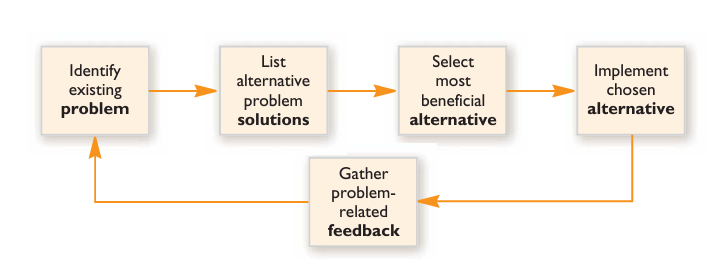
\includegraphics[scale=1.0]{Model_of_DM.png}
  \caption{Model of the decision-making process \cite{model_decision_making}}
  % \label{fig:boat1}
\end{figure}

To address uncertain decision-making, we've devised a structured framework with these key steps:
\subsubsection{Start by Defining the Problems and Goals}
Kepner and Tregoe developed a problem analysis method, emphasizing the importance of the first stage of decision-making—identifying the problem. According to their framework, the precision with which the problem is defined has a significant impact on the decision's quality\cite{lunenburg2010decision}. The method of problem analysis includes: 
\\(1) problem identification,\\(2) definition of what the problem is and is not,\\ (3) prioritizing the problem, and \\(4) testing for cause-effect relationships.
\\
\\\textit{The Importance of Well-Defined Problems:} In software engineering, poorly defined problems frequently lead to project failure. It is critical to devote time to defining problems, comprehending stakeholder needs, identifying potential risks, and aligning problems with project objectives. This step helps to avoid "bikeshedding," which occurs when discussions focus on implementation details before agreeing on the need for a solution.



% Your content on defining problems and goals
\subsubsection{Collect Information from Multiple Sources}
% Your content on collecting information from multiple sources
Effective software engineering decision-making requires gathering insights and perspectives from a variety of stakeholders, including developers, designers, product owners, and end users. Collaborative input aids in the formation of a comprehensive view of the problem.

\textit{Collaboration Among Stakeholders:} A lack of understanding of business strategy and poor communication between business-level, product-level, and project-level stakeholders is identified as significant problems, particularly when the customer is external to the organization.\cite{CUNHA2016947}
Collaboration is essential in software engineering. Learning to gather information from a variety of sources, such as team members and clients, is essential to make good decisions.

\subsubsection{Outline the Options}
% Your content on outlining options
In decision-making under uncertainty, identifying a broad range of alternatives and evaluating them against set criteria is crucial. This process involves considering both conventional and unconventional options, ensuring they align with core requirements despite uncertain conditions.\cite{fulop2005introduction}Ultimately, the focus shifts from seeking perfect solutions to choosing options that offer adaptability and risk mitigation, prioritizing flexibility in response to the unpredictability inherent in uncertain environments.

\textit{Accepting Creativity:} Embracing creativity in uncertain decision-making scenarios means welcoming innovative solutions and fresh perspectives. This approach enhances adaptability and problem-solving effectiveness in complex and ambiguous situations.

\subsubsection{Integrating Intuition in Managerial Decisions}
In managerial decision-making under uncertainty, a combination of structured and intuitive approaches is essential. Traditional, rule-based decision-making is effective for routine scenarios, while in uncertain situations, intuition, emotional judgment, and imitative strategies play a crucial role.Daniel Kahneman and Amos Tversky were awarded the Nobel Prize for further examining the role of intuition in decision making.

\textit{Decisions in complex situations:} These alternate strategies emphasize flexibility, adaptability, and creativity, allowing for effective decisions in complex or unprecedented situations. This balanced approach leverages both conventional methods and individual judgment to enhance decision-making effectiveness.\cite{rachel2011common}

\subsubsection{Be Cognizant of the Risks}
% Your content on being cognizant of the risks
Managers exhibit diverse attitudes towards risk, affecting their decision-making processes. While some managers view risk-taking as necessary for organizational progress, others are more cautious, focusing on minimizing potential negative outcomes.\cite{riabacke2006managerial}
\newline
\newline
\textit{Risk Management as a Skill:} When making decisions, especially in uncertain contexts, it's essential to consider the potential consequences and associated risks. This approach encourages moving beyond initial fears and gut reactions, enabling a more comprehensive evaluation of possible outcomes. By contemplating the best, worst, and intermediate scenarios, decision-makers can gain a clearer understanding of the full spectrum of possibilities. This method is particularly useful in complex environments where decisions carry significant weight and uncertainty, as it allows for a more informed and balanced consideration of risks and rewards. This approach not only enhances the quality of decision-making but also contributes to more strategic and resilient organizational planning.

\subsubsection{Consider doing experiments instead of making decisions}
The concept of treating decisions as temporary experiments aligns with the continuous nature of decision-making. It recognizes that decisions are steps in an ongoing process, requiring periodic reassessment and adjustment.\cite{lunenburg2010decision} By setting specific time frames to reevaluate decisions, it facilitates a dynamic and adaptive approach, allowing for timely responses to evolving situations and the effectiveness of chosen strategies.

\subsection{Decision Making Tools}
\subsubsection{Probability Theory}
Probability theoryis a decision-making tool used in risk situations—situations in which decision makers are not completely sure of the outcome of an implemented alternative.Probability refers to the likelihood that an event or outcome will actually occur.It is estimated by calculating an expected value for each alternative considered.Specifically,the expected value (EV) for an alternative is the income (I) that alternative would produce,multiplied by its probability of producing that income (P).In formula form,\textbf{EV= I X P}. Decision makers generally choose and implement the alternative with the highest expected value.\cite{mosier1989expected}
\subsubsection{Decision Trees}
A decision tree is a graphic decision-making tool typically used to evaluate decisions involving a series of steps.

\subsubsection{Approach Used in Case Studies}

\textbf{Case Study 1:}
The decision-making approach involved a Probabilistic Model inspired by Bernoulli and Laplace's work. It included a Risk Assessment where experts assigned probabilities to uncertainties for each sourcing option. A Quantitative Assessment measured supply chain disruption scale, and a Financial Implications Analysis translated probabilities into potential supply loss/gain and margins. This comprehensive analysis enabled a strategic evaluation of each alternative's financial impact.
\newline\newline
\textbf{Case Study 2:}
The approach involved identifying the problem of low ratings, listing potential solutions related to guest quality, writing, and advertising, evaluating and selecting the most feasible solution based on problem identification, and finally, implementing and monitoring the chosen solution's effectiveness.


\section{Results}
\subsection{Results of the Approach used in Case Studies}
\textbf{1. Case Study 1:} The decision-making process involved quantifying consequences for each sourcing alternative, assessing supply security, brand risks, and geopolitical/environmental factors. The decisive entry into Countries A and B was driven by a 70\% chance of higher profits. The phased approach prioritized ramping up in Country B initially, delaying evaluation of the political situation in Country A. Concurrently, consideration was given to automation for reshoring, reflecting a versatile strategy amid global sourcing complexities.
\newline
\newline
\textbf{Case Study 2:} The initial reorganization resulted in low ratings and a negative public response. Subsequently, the prime-time Leno show was canceled, leading to Jay Leno's reinstatement as the host of "The Tonight Show." In response, Conan O'Brien departed NBC, receiving a severance package, and later joined TBS.
\subsection{Limitations:}
In Case Study 1, the model accuracy relies on input data quality; probabilistic models may overlook dynamic geopolitical/environmental risks, and the process may not address unquantifiable factors like sudden market shifts or brand perception changes.
\\
\\
In Case Study 2, limitations include predicting viewer preferences, market response, talent dynamics, and public perception inadequately, with limited flexibility for unexpected outcomes. 
\subsection{Suggestions}
1. To enhance probabilistic decision-making in Case Study 1, the strategy involves prioritizing data excellence through regular updates and diverse sources. Embracing dynamic modeling, including scenario and sensitivity analyses, ensures preparedness for unforeseen events. Additionally, addressing unquantifiable risks involves integrating qualitative insights and stakeholder engagement.
\\
2. To overcome limitations in Case Study 2, enhance market research, implement flexible decision models, and engage stakeholders regularly. For future decisions, apply probabilistic models, utilize decision trees, and incorporate group decision-making processes for comprehensive analysis and consensus building.

% Your content on conditions where the framework is effective
\subsection{Constraints}
In a rapidly changing world, decision-making faces the challenge of evolving information. Strategies effective in stable conditions may falter in dynamic environments, necessitating a reevaluation of how decisions are made. Adapting to the changing nature of information is crucial for maintaining decision quality, underscoring the need for tools and approaches tailored to these shifting dynamics.\cite{walton2020limitations}
% Your content on constraints
% \section{Quality Assessment}
% % Your content on quality assessment

\section{Conclusion and Future Work}
\subsection{Future Work}
\subsubsection{Necessity of Adaptive Strategies in Decision-Making}
In decision-making within uncertain and rapidly changing environments, a shift towards adaptive strategies is crucial. Traditional methods often fall short, requiring decision-makers to be agile and flexible. Embracing uncertainty as a natural aspect of decision-making and maintaining a clear focus on objectives can guide more informed and confident choices. Utilizing a range of techniques like scenario planning, prototyping, experimentation, and risk management proves beneficial in navigating these challenges. Collaboration also plays a key role. Overall, agility and adaptability are vital in ensuring effective decision-making in the face of evolving information and dynamic conditions.
\subsubsection{Decision making in Agile Development}
To further advance the field of decision-making under uncertainty, it's essential to focus on strategic alignment in agile methodologies, enhance the adaptability of sprint planning and execution, and reinforce team commitment and autonomy.\cite{drury2011decision} Deepening the understanding through methodological advancements, particularly through comprehensive studies of Agile Software Development teams, is crucial. Additionally, evaluating the impact of various decision-making strategies on project performance in uncertain environments can offer valuable insights for refining and optimizing agile processes.
% Your content on limitations
\subsection{Conclusion}
Decision making under uncertainty and risk is a complicated and difficult process, but managers may make informed and confident judgements by employing the appropriate tactics and procedures. A variety of techniques, including as scenario planning, prototyping, experimentation, risk management, and teamwork, can assist managers negotiate uncertainty and risk in their decision making. Furthermore, managers may become effective in decision making under uncertainty by accepting ambiguity as a normal part of the process and having a clear focus on objectives. 
Embracing  adaptability, combined with a continuous learning mindset, can transform uncertainty from a challenge into an opportunity for innovation and growth.
% Your content on the Agile perspective
% \chapter{References}
\bibliographystyle{IEEEtran}
\addcontentsline{toc}{section}{References}
\begin{thebibliography}{9}
\section*{Citations}
\bibitem{vroom1973leadership}
Vroom, V. H., \& Yetton, P. W. (1973). \textit{Leadership and decision-making.} University of Pittsburgh Press.

\bibitem{lunenburg2010decision}
Lunenburg, F. C. (2010). \textit{The decision-making process}. National Forum of Educational Administration \& Supervision Journal, 27(4).

\bibitem{riabacke2006managerial}
Riabacke, A. (2006). \textit{Managerial Decision Making Under Risk and Uncertainty}. IAENG International Journal of Computer Science, 32(4).

\bibitem{forman2001decision}
Forman, E. H. and Selly, M. A. (2001). \textit{Decision by Objectives: How to Convince Others that You are Right}. World Scientific. ISBN: 9789810241438. 

\bibitem{LIPSHITZ1997149}
 Lipshitz, R., and Strauss, O. (1997). \textit{Coping with Uncertainty: A Naturalistic Decision-Making Analysis}. \textit{Organizational Behavior and Human Decision Processes}, 69(2), 149-163. ISSN: 0749-5978. 
% DOI:\url{https://doi.org/10.1006/obhd.1997.2679}. URL: \url{https://www.sciencedirect.com/science/article/pii/S0749597897926790}.

\bibitem{ahmed2012theories}
Ahmed, M. T., and Omotunde, H. (2012). \textit{Theories and Strategies of Good Decision Making}. \textit{International Journal of Scientific \& Technology Research}, 1(10), 51-54.

\bibitem{rachel2011common}
Dinur, A. R. (2011). \textit{Common and Uncommon Sense in Managerial Decision Making under Task Uncertainty}. \textit{Management Decision}, 49(5), 694-709. Publisher: Emerald Group Publishing Limited.

\bibitem{CUNHA2016947}
Cunha, J. A. O. G., Moura, H. P., and Vasconcellos, F. J. S. (2016). \textit{Decision-making in Software Project Management: A Systematic Literature Review}. \textit{Procedia Computer Science}, 100, 947-954. ISSN: 1877-0509. 
%DOI: \url{https://doi.org/10

\bibitem{fulop2005introduction}
F{\"u}l{\"o}p, J{\'a}nos (2005). \textit{Introduction to Decision Making Methods}. In \textit{BDEI-3 Workshop, Washington}, pp. 1-15.

\bibitem{walton2020limitations}
Walton, P. (2020). \textit{The Limitations of Decision-Making}. \textit{Information}, 11(12), 559. Publisher: MDPI.

\bibitem{drury2011decision}
Drury, M., Conboy, K., and Power, K. (2011). \textit{Decision Making in Agile Development: A Focus Group Study of Decisions and Obstacles}. In \textit{2011 Agile Conference}, pp. 39-47. Organization: IEEE.

\bibitem{taghavifard9decision}
Taghavifard, MT, Damghani, K Khalili, and Moghaddam, R Tavakkoli (2009). \textit{Decision Making under Uncertain and Risky Situations}. In \textit{Society of Actuaries}, pp. 1-31.

\bibitem{owczarskireview}
Owczarski, Kimberly. (Year). \textit{A Review of Contemporary Media}.


\section*{Appendix}
\bibitem{mathiasMeyer}
Mathias Meyer. \textit{Dealing with Uncertainty}. In \textit{Collective Wisdom from the Experts}.

\bibitem{model_decision_making}
\textit{Making Decisions}, Cairo University Scholars.

\bibitem{mosier1989expected}
Mosier, R. C. (1989). \textit{Expected Value: Applying Research to Uncertainty}. In \textit{Appraisal Journal (July 1989)}.

\bibitem{Itsomerz2014}
Itsomerz. (2014, March 11).\textit{ Project risks – people do not recognize uncertainty as risk until it’s very much certain. }Omerz.

\begin{table}[h]
\centering
\begin{tabular}{|p{0.2\linewidth}|p{0.35\linewidth}|p{0.35\linewidth}|}
\hline
\textbf{Section} & \textbf{Prompts} & \textbf{Corrections} \\
\hline
Report & ``Review for grammatical errors.'' & Suggestions for grammatical improvements. \\
\hline
Results & ``Proofread  for clarity in discussion.'' & Proposed restructuring for better flow in discussion section. \\
\hline
\end{tabular}
\caption{Log of interactions with ChatGPT for proofreading and corrections.}
\label{tab:chatgpt-log}
\end{table}

% Add more citations as needed

\end{thebibliography}
\section*{Acknowledgement}
I extend my gratitude to OpenAI's ChatGPT for its assistance in proofreading and correcting grammatical errors throughout the development of this project. Additionally, I acknowledge the role of Google Scholar in facilitating the discovery of pertinent case studies that significantly enriched the research. Details of the interactions with ChatGPT and the specific case studies sourced from Google Scholar are documented in the appendix.
\end{document}
